\documentclass[10pt]{article}
\usepackage[utf8]{inputenc}
\usepackage[T1]{fontenc}
\usepackage{amsmath}
\usepackage{amsfonts}
\usepackage{amssymb}
\usepackage[version=4]{mhchem}
\usepackage{stmaryrd}
\usepackage{graphicx}
\usepackage[export]{adjustbox}
\graphicspath{ {./images/} }

\title{Water Distribution Operator Requirements }

\author{}
\date{}

\begin{document}
\begin{enumerate}
\item The basic goal for water treatment is to \rule{2cm}{0.3pt}.\\
a.  Protect public health\\
b.  Make it clear\\
c.  Make it taste good\\
d.  Get stuff out\\

\item Greensand can be operated in either \rule{2cm}{0.5pt} regeneration or \rule{2cm}{0.5pt} regeneration modes.\\
a.  Continuous or intermittent\\
b.  Fast or slow\\
c.  Hot or cold\\
d.  Constant or unusual\\

\item The two most common types of chlorine disinfection by-products include:\\
a.  TTHM and HAA5\\
b.  TTHA of HMM5\\
c.  Turbidity and color\\
d.  Chloride and fluoride\\

\item GAC contactors are used to reduce the amount of \rule{2cm}{0.5pt} contaminants in water.\\
a.  Inorganic\\
b.  Turbidity\\
c.  Particle\\
d.  Organic\\

\item List the five types of surface water filtration systems.\\
a.  Bag filtration, cartridge filtration, fine filtration, coarse filtration, media filtration\\
b.  Conventional treatment, direct filtration, slow sand filtration, diatomaceous earth filtration, membrane filtration\\
c.  Turbidity filtration, color filtration, bag filtration, fine filtration, media filtration\\
d.  None of the above\\

\item Describe two primary methods used to control taste and odor?\\
a.  Oxidation and adsorption\\
b.  Filtration and sedimentation\\
c.  Mixing and coagulation\\
d.  Sedimentation and clarification\\

\item The adsorption process is used to remove:\\
a.  Organics or inorganics\\
b.  Bugs or salts\\
c.  Organisms or dirt\\
d.  Color or particles\\

\item The solid that adsorbs a contaminant is called the:\\
a.  Adsorbent\\
b.  Adsorbate\\
c.  Sorbet\\
d.  Rock\\

\item What is a method of reducing hardness?\\
a.  Softening\\
b.  Hardening\\
c.  Lightning\\
d.  Flashing\\


\item What percentage of all the earth's water is readily available as a potential drinking water supply in the form of lakes, rivers, and near-surface groundwater?\\
a.  97\%\\
b.  50\%\\
c.  2\%\\
d.  1\%\\
e.  0.34\%\\

\item To  prevent the entry of surface contamination into a well is the purpose of\\
a.  The well casing\\
b.  The water table\\
c.  The louvers or slots\\
d.  Well development\\
e.  The  annular grout seal\\

\item An aquifer that is located underneath an aquiclude is called\\
a.  An unconfined aquifer\\
b.  A confined aquifer\\
c.  A water table\\
d.  Unreachable groundwater\\
e.  An Artesian spring\\

\item The process by which water changes from the gas to the liquid phase is termed\\
a.  Condensation\\
b.  Evaporation\\
c.  Percolation\\
d.  Precipitation\\
e.  Runoff\\

\item The free surface of the water in an unconfined aquifer is known as the\\
a.  Pumping water level\\
b.  Artesian spring\\
c.  Water table\\
d.  Drawdown\\
e.  Percolation\\


\item  The type of organisms that can cause disease are said to be \rule{2cm}{0.3pt}
microorganisms.\\
a.  Bad\\
b.  Pathogenic\\
c.  Undesirable\\
d.  Sick\\

\item  Four types of aesthetic contaminants in water include the following:\\
a.  Odor, turbidity, color, hydrogen sulfide gas\\
b.  Pathogens, microorganisms, arsenic, disinfection by-products\\
c.  Odor, color, turbidity, hardness\\
d.  Color, pathogens, metals, organics\\


\item  What is the purpose of adding fluoride to drinking water?\\
a.  Increase tooth decay\\
b.  Reduce tooth decay\\
c.  Make teeth white\\
d.  Government conspiracy\\

\item  The test used to determine the effectiveness of disinfection is called the:\\
a.  Coliform bacteria test\\
b.  Color test\\
c.  Turbidity test\\
d.  Particle test\\

\item  Turbidity is measured as:\\
a.  Mg/L
b.  mL\\
c.  gpm\\
d.  NTU\\

\item  Giardia and cryptosporidium are a type of:\\
a.  Mineral\\
b.  Organism\\
c.  Color\\
d.  Bird\\



\item Head is measured in\\
a. absolute pressure.\\
b. gauge pressure.\\
c. feet.\\
d. foot-pounds.

\item A plat is
a. a map.\\
b. a corrosion point on a pipe.\\
c. organelle found in some protozoans.\\
d. a highly corrosive soil type.

\item Which type of valve will prevent the collapse of a pipe?\\
a. Pressure-relief valve\\
b. Needle valve\\
c. Pinch valve\\
d. Air-and-vacuum relief valve

  \item The highest degree of protection for the exterior of a coated steel pipe is\\
a. cathodic protection.\\
b. bituminous materials.\\
c. plastic coatings.\\
d. polyethylene tapes.

  \item At which time of day is the age of the water stored in the distribution system the highest?\\
a. Early morning\\
b. Late morning\\
c. Early afternoon\\
d. Late evening

  \item The amount of liquid that can be raised vertically by a given pressure is called\\
a. pressure head.\\
b. total head.\\
c. velocity head.\\
d. pump head.

  \item The amount of energy in feet that a pump supplies to a fluid is called\\
a. velocity head.\\
b. pump head.\\
c. total head.\\
d. pressure head.

  \item The C-value is a measure of a pipe's wall\\
a. smoothness.\\
b. smoothness giving even flow.\\
c. smoothness that retards turbulent flow.\\
d. roughness that retards flow due to friction.

  \item Which one of the following is a type of joint for ductile iron piping?\\
a. Expansion joint\\
b. Push-on joint\\
c. Bell and spigot with rubber o-ring\\
d. Rubber gasket joint

  \item The correct protective methods for backflow-prevention devices in order of decreasing effectiveness are\\
a. air gap, VB, RPZ, and DCVA.\\
b. air gap, VB, DCVA, and RPZ.\\
c. air gap, RPZ, VB, and DCVA.\\
d. air gap, RPZ, DCVA, and VB.


  \item One of chlorine's advantages is that it\\
a. is not influenced much by $\mathrm{pH}$ changes.\\
b. does not produce chlorinated by-products.\\
c. has a persistent residual.\\
d. does not cause taste and odor problems.

  \item Chlorine gas is times heavier than air.\\
a. $\quad 1.5$\\
b. $\quad 2.5$\\
c. $\quad 3.5$\\
d. $4.5$ 

	\item After a water storage tank has been chlorinated, which bacteriological test must prove negative before the tank is put back into service?\\
a. Gram negative test\\
b. HPC test\\
c. Coliform test\\
d. Chloramine test

  \item Which is the best and most reliable method for finding a very small chlorine leak?\\
a. Use soap on possible areas of leak and watch for bubbles\\
b. Use a strong ammonia solution on a cloth swab and place it by the suspected leak\\
c. Use methane gas and watch for a dark brown smoke\\
d. Use a chlorine gas detector and place it next to any area suspected of leaking

  \item The minimum required free chlorine residual anywhere in the distribution system is\\
a. a detectable level.\\
b. $\quad 0.2 \mathrm{mg} / \mathrm{L}$.\\
c. $0.4 \mathrm{mg} / \mathrm{L}$.\\
d. $0.5 \mathrm{mg} / \mathrm{L}$.

  \item Sodium hypochlorite $(\mathrm{NaOCl})$ solution is available with available chlorine.\\
a. 2 to $5 \%$\\
b. 5 to $20 \%$\\
c. 25 to $50 \%$\\
d. 50 to $70 \%$

  \item Booster chlorination is chlorine added\\
a. in the coagulation mixing chamber.\\
b. before the filters.\\
c. at the clearwell.\\
d. somewhere in the distribution system.

  \item According to AWWA Standard C651, disinfection of water mains requires 24-hour exposure to which minimum free chlorine residual?\\
a. $10 \mathrm{mg} / \mathrm{L}$\\
b. $25 \mathrm{mg} / \mathrm{L}$\\
c. $50 \mathrm{mg} / \mathrm{L}$\\
d. $100 \mathrm{mg} / \mathrm{L}$

  \item Which must be measured at least at the same time and at the same sampling points in the distribution system that total coliforms are sampled for a water system that only uses surface water?\\
a. $\mathrm{pH}$\\
b. Langelier Index\\
c. Residual disinfectant concentration\\
d. Heterotrophic bacteria 

\item Hypochlorous acid is\\
a. a weak acid.\\
b. a strong acid.\\
c. easily dissociatable.\\
d. hydrophobic.

  \item First draw samples for the analysis of lead and copper water must be collected from taps where the water has stood motionless in the plumbing for at least\\
a. 4 hours.\\
b. 6 hours.\\
c. 8 hours.\\
d. 24 hours.

  \item Samples to be tested for coliforms are collected in plastic bottles that must contain\\
a. sodium thiocarbonate.\\
b. sodium thiooxalate.\\
c. sodium thiosulfate.\\
d. sodium thiocyanate.

  \item The volume of a sample for coliform compliance is\\
a. $100 \mathrm{~mL}$.\\
b. $200 \mathrm{~mL}$.\\
c. $300 \mathrm{~mL}$.\\
d. 0 ; there is no volume compliance for coliforms.

  \item If a water sample is not analyzed immediately for chlorine residual, it is acceptable if it is analyzed within\\
a. 10 minutes.\\
b. 15 minutes.\\
c. 20 minutes.\\
d. 30 minutes.

  \item Which may be substituted for the analysis of residual disinfectant concentration, when total coliforms are also sampled at the same sampling point?\\
a. Heterotrophic plate count (HPC)\\
b. Fecal coliforms\\
c. Giardia lamblia\\
d. Combined chlorine

  \item Which water quality parameter requires a grab sample because it cannot be collected as a composite sample?\\
a. $\mathrm{pH}$\\
b. Iron\\
c. Nitrate\\
d. Zinc 

	\item One chemical characteristic of an acid is that it will\\
a. accept an electron pair.\\
b. donate an electron pair.\\
c. accept a proton.\\
d. accept a neutron.

  \item Which chemical contains calcium?\\
a. Soda ash\\
b. Lime\\
c. Caustic soda\\
d. Sodium bicarbonate

  \item The best choice to collect a water sample from a customer's faucet in regards to a complaint would be a\\
a. faucet without threads.\\
b. faucet that can swivel.\\
c. single-lever handle faucet.\\
d. faucet with an aerator.

  \item When measuring for free chlorine residual, which method is the quickest and simplest?\\
a. DPD color comparater\\
b. Orthotolidine method\\
c. Amperometric titration\\
d. 1, 2 nitrotoluene di-amine method

  \item It is standard practice to install fire hydrants on mains that are at a minimum or larger.\\
a. 6 inches\\
b. 8 inches\\
c. 10 inches\\
d. 12 inches

  \item A corporation stop is used for a\\
a. service line.\\
b. pump discharge line.\\
c. tank inlet.\\
d. tank outlet.

  \item When PVC pipe is stacked loose, it should not be stacked more than how high?\\
a. $2.0$ feet\\
b. $3.0$ feet\\
c. $5.0$ feet\\
d. $7.5$ feet

  \item Which is the most common cause for pipe joint failure (leaking) in newly laid pipe\\
a. The use of a cracked gasket\\
b. Not pushing the spigot end the full distance into the bell\\
c. Not having the joint completely clean\\
d. An incorrect trench bedding angle

  \item Which should be installed at a dead-end water main?\\
a. Vacuum valve\\
b. Air valve\\
c. Blowoff valve\\
d. Water quality sampling station

  \item Compression fittings used with copper or plastic tubing seal by means of a\\
a. beveled sleeve.\\
b. compression ring.\\
c. compressed beveled gasket.\\
d. compressed o-rings located at either end of the fitting's beveled neck. 

  \item The breaking of a buried pipe when it is unevenly supported is called\\
a. stress breakage.\\
b. shear breakage.\\
c. beam breakage.\\
d. flexural breakage.

  \item Thrust from a water surge almost always acts pushes against. to the inside surface that it\\
a. vertically\\
b. horizontally\\
c. perpendicular\\
d. vertically and horizontally

  \item Which thrust control is easy to use, especially in locations where existing utilities or structures are numerous?\\
a. Restraining fittings\\
b. Tie rods\\
c. Thrust anchors\\
d. Thrust blocks

  \item The backfill material for a pipe installation should contain enough to allow for thorough compaction.\\
a. moisture\\
b. sand\\
c. gravel\\
d. mixed sizes

  \item The "heart" of a pump is called the\\
a. volute case.\\
b. impeller.\\
c. motor.\\
d. pump.

  \item Which device serves the same function as the packing?\\
a. Inline suction gland\\
b. Packing gland\\
c. Mechanical seal\\
d. Lantern seal

  \item Which is used to stop air leakage into the casing around a pump shaft?\\
a. Packing gland\\
b. Lantern ring\\
c. Seals\\
d. Shaft sleeves

  \item Which is at the top of a stuffing box?\\
a. Packing gland\\
b. Lantern ring\\
c. Mechanical seal\\
d. Seal cage 

	\item Which assembly holds the lantern ring and packing?\\
a. Shaft assembly\\
b. Casing ring assembly\\
c. Packing gland casing\\
d. Stuffing box

  \item Which of the following prevents the impeller of a pump from turning on the shaft?\\
a. Lock nut on threaded shaft\\
b. Key\\
c. Steel pin\\
d. Caliper pin

  \item Which type of valve is used to isolate a pump on the suction side?\\
a. Butterfly valve\\
b. Globe valve\\
c. Gate valve\\
d. Ball valve

  \item Water hammer can be described as\\
a. particle waves.\\
b. acoustic waves.\\
c. rogue waves.\\
d. longitudinal waves.

  \item When fully opened, which valve will have the highest head loss?\\
a. Gate valve\\
b. Plug valve\\
c. Globe valve\\
d. Ball valve

  \item Which type of pressure sensor uses a wire fastened to a diaphragm?\\
a. Bellows sensor\\
b. Strain gauge\\
c. Helical sensor\\
d. Diaphragm element

  \item Why is it so important to monitor the speed of a variable-speed pump?\\
a. To prevent excessive temperatures from developing\\
b. To prevent vibration from developing\\
c. To prevent speed oscillation from occurring\\
d. To prevent cavitation from occurring

  \item Which basic electrical unit is used to measure a material's opposition to the flow of electricity?\\
a. Ampere\\
b. Ohm\\
c. Volts\\
d. Resistance or impedance

  \item The first oil change on a new pump should be done\\
a. after the first two weeks of operation.\\
b. after one month of operation.\\
c. after three months of operation.\\
d. after six months of operation.

  \item How often should the temperature of centrifugal pump motor bearings be checked with a thermometer?\\
a. Every day\\
b. Once a week\\
c. Twice a month\\
d. Once a month

  \item All sensors that respond to liquid pressure will perform poorly if $\operatorname{enter}(\mathbf{s})$ the sensor.\\
a. air\\
b. corrosive chemicals from water treatment processes\\
c. corrosive chemicals from piping\\
d. iron bacteria

  \item Packing replacement is usually performed when\\
a. water leakage sprays out of the pump housing.\\
b. no further tightening can be done on the packing gland.\\
c. the packing gland bolts are exposed by more than $2^{1 / 2}$ inches above the nut.\\
d. the packing has completely disintegrated. 

\item Which device changes alternating current to direct current by allowing the electric current to flow in one direction but blocking flow in the opposite direction?\\
a. Regulator\\
b. Converter\\
c. Inverter\\
d. Rectifier

  \item To ease installation of impeller wear rings, they can be\\
a. lubricated with a light oil.\\
b. greased with lithium.\\
c. heated.\\
d. cooled.

  \item Packing is designed to\\
a. add lubricant to the shaft.\\
b. expand and deteriorate with normal use.\\
c. protect the shaft.\\
d. wear and deteriorate with normal use.

  \item Bearings on a line shaft turbine can be lubricated with\\
a. oil or water.\\
b. grease or oil.\\
c. lithium or grease.\\
d. graphite or grease.

  \item Which agency sets legal limits on the concentration levels of harmful contaminants in potable water distributed to customers?\\
a. National Primary Drinking Water Regulations\\
b. United States Environmental Protection Agency\\
c. United States Public Health Service\\
d. Occupational Health and Safety Organization

  \item Which violations are the most serious?\\
a. Tier I\\
b. Tier II\\
c. Tier III\\
d. Tier IV

  \item A positive fecal coliform test must be reported to the primacy agency within\\
a. 8 hours.\\
b. 12 hours.\\
c. 24 hours.\\
d. 48 hours.

  \item The number of monthly distribution system bacteriological samples required is\\
a. based on water withdrawal permit limit.\\
b. based on system size.\\
c. based on population served.\\
d. different for each state.

  \item Which is the approximate angle of repose for average soils when using the sloping method for the prevention of cave-ins? (Note: horizontal to vertical distance, respectively)\\
a. $0.5: 1.0$\\
b. $1.0: 1.0$\\
c. $1.5: 1.0$\\
d. $2.0: 1.0$

  \item Which is the Maximum Contaminant Level for total trihalomethanes (TTHMs)?\\
a. $0.040 \mathrm{mg} / \mathrm{L}$\\
b. $\quad 0.060 \mathrm{mg} / \mathrm{L}$\\
c. $0.080 \mathrm{mg} / \mathrm{L}$\\
d. $0.100 \mathrm{mg} / \mathrm{L}$ 

\item A system that fails to collect water samples in their distribution system would fall under which public notification requirement?\\
a. Tier I\\
b. Tier II\\
c. Tier III\\
d. Tier IV

  \item Under the Surface Water Treatment Rule, disinfection residuals must be collected at the same location in the distribution system as\\
a. coliform samples.\\
b. total trihalomethanes.\\
c. disinfection by-products.\\
d. alkalinity, conductivity, and $\mathrm{pH}$ for corrosion studies.

  \item Iron can cause "red water" and thus customer complaints when its concentration is above its secondary maximum contaminant level of\\
a. $0.01 \mathrm{mg} / \mathrm{L}$.\\
b. $\quad 0.05 \mathrm{mg} / \mathrm{L}$.\\
c. $0.10 \mathrm{mg} / \mathrm{L}$.\\
d. $0.30 \mathrm{mg} / \mathrm{L}$.

  \item Which chemical may encourage the growth of algae and microorganisms?\\
a. Lime\\
b. Sodium bicarbonate\\
c. Sodium hydroxide\\
d. Zinc orthophosphate

  \item A well yields 2,840 gallons in exactly 20 minutes. What is the well yield in gpm?\\
a. $140 \mathrm{gpm}$\\
b. 142 gpm\\
c. $145 \mathrm{gpm}$\\
d. $150 \mathrm{gpm}$

  \item Convert $37.4$ degrees Fahrenheit to degrees Celsius.\\
a. $3.0^{\circ} \mathrm{C}$\\
b. $5.3^{\circ} \mathrm{C}$\\
c. $7.9^{\circ} \mathrm{C}$\\
d. $9.7^{\circ} \mathrm{C}$

  \item What is the area of a circular tank pad in $\mathrm{ft}^{2}$, if it has a diameter of $102 \mathrm{ft}$ ?\\
a. $6,160 \mathrm{ft}^{2}$\\
b. $\quad 6,167 \mathrm{ft}^{2}$\\
c. $8,170 \mathrm{ft}^{2}$\\
d. $8,200 \mathrm{ft}^{2}$

  \item What is the pressure $1.85$ feet from the bottom of a water storage tank if the water level is $28.7$ feet?\\
a. $11.6 \mathrm{psi}$\\
b. $\quad 12.4 \mathrm{psi}$\\
c. $\quad 62.0 \mathrm{psi}$\\
d. $66.3$ psi

  \item Calculate the well yield in gpm, given a drawdown of $14.1 \mathrm{ft}$ and a specific yield of 31 $\mathrm{gpm} / \mathrm{ft}$.\\
a. $2.2 \mathrm{gpm}$\\
b. $7.3 \mathrm{gpm}$\\
c. $45.1 \mathrm{gpm}$\\
d. $440 \mathrm{gpm}$

  \item How many gallons are in a pipe that is $18.0$ in. in diameter and $1,165 \mathrm{ft}$ long?\\
a. 2,060 gal\\
b. 10,300 gal\\
c. $15,400 \mathrm{gal}$\\
d. 17,200 gal 

  \item A water tank with a capacity of $5.75$ million gallons (mil gal) is being filled at a rate of 2,105 gpm. How many hours will it take to fill the tank?\\
a. $31.6 \mathrm{hr}$\\
b. $37.8 \mathrm{hr}$\\
c. $42.9 \mathrm{hr}$\\
d. $45.5 \mathrm{hr}$

  \item Determine the detention time in hours for the following water treatment system:
\begin{itemize}
  \item Distribution pipe from water plant to storage tank is $549 \mathrm{ft}$ in length and 14 in. in diameter

  \item Storage tank averages 2,310,000 gal of water at any given time

  \item Flow through system is $6.72 \mathrm{mgd}$\\
  
  \end{itemize}
a. $7.2 \mathrm{hr}$\\
b. $7.4 \mathrm{hr}$\\
c. $8.0 \mathrm{hr}$\\
d. $8.3 \mathrm{hr}$

  \item Convert $28.7$ cubic feet per second (cfs) to gallons per minute (gpm).\\
a. $12,477 \mathrm{gpm}$\\
b. $12,700 \mathrm{gpm}$\\
c. $12,880 \mathrm{gpm}$\\
d. $12,900 \mathrm{gpm}$

  \item Convert 16,912,000 liters to acre-feet.\\
a. $13.7$ acre-ft\\
b. $41.5$ acre-ft\\
c. $51.9$ acre-ft\\
d. 767 acre-ft

  \item Convert $-22.6^{\circ} \mathrm{C}$ to degrees Fahrenheit.\\
a. $-4.6^{\circ} \mathrm{F}$\\
b. $-8.7^{\circ} \mathrm{F}$\\
c. $-11.8^{\circ} \mathrm{F}$\\
d. $-12.8^{\circ} \mathrm{F}$

  \item A sodium hypochlorite solution contains $11.3 \%$ hypochlorite. Calculate the $\mathrm{mg} / \mathrm{L}$ hypochlorite in the solution.\\
a. $11.3 \mathrm{mg} / \mathrm{L}$ sodium hypochlorite\\
b. $1,130 \mathrm{mg} / \mathrm{L}$ sodium hypochlorite\\
c. $11,300 \mathrm{mg} / \mathrm{L}$ sodium hypochlorite\\
d. $113,000 \mathrm{mg} / \mathrm{L}$ sodium hypochlorite

  \item Records for a pump show that on June 1st at exactly 9:00 a.m. the number of pumped gallons was $71,576,344$ and on July 1st at exactly 9:00 a.m. it was 72,487,008 gallons. Determine the average gallons pumped per day (gal/day) for this month to the nearest gallon.\\
a. $18,605 \mathrm{gal} / \mathrm{day}$\\
b. $25,875 \mathrm{gal} / \mathrm{day}$\\
c. $30,355 \mathrm{gal} / \mathrm{day}$\\
d. $34,325 \mathrm{gal} /$ day 

\item If chlorine is being fed at a rate of $260 \mathrm{lb} /$ day for a flow rate of $23 \mathrm{cfs}$, which should be the adjustment on the chlorinator when the flow rate is decreased to $16 \mathrm{cfs}$, if all other water parameters remain the same?\\
a. $160 \mathrm{lb} /$ day\\
b. $180 \mathrm{lb} / \mathrm{day}$\\
c. $310 \mathrm{lb} /$ day\\
d. $370 \mathrm{lb} / \mathrm{day}$

  \item Calculate the diameter of a clarifier with a circumference of $215 \mathrm{ft}$.\\
a. $34.8 \mathrm{ft}$\\
b. $56.7 \mathrm{ft}$\\
c. $\quad 68.5 \mathrm{ft}$\\
d. $\quad 76.2 \mathrm{ft}$

  \item Determine the depth of water in a reservoir, if the psi is 31.9.\\
a. $13.8 \mathrm{ft}$ deep\\
b. $24.9 \mathrm{ft}$ deep\\
c. $45.6 \mathrm{ft}$ deep\\
d. $73.7 \mathrm{ft}$ deep

  \item Calculate the area of a tank, if the tank's radius is $39.8 \mathrm{ft}$.\\
a. $4,970 \mathrm{ft}^{2}$\\
b. $\quad 5,670 \mathrm{ft}^{2}$\\
c. $7,820 \mathrm{ft}^{2}$\\
d. $9,940 \mathrm{ft}^{2}$

  \item Determine the specific gravity (SG) of an unknown liquid, if the density of the liquid is $70.9 \mathrm{lb} / \mathrm{ft}^{3}$.\\
a. 1.05 SG\\
b. 1.14 SG\\
c. $1.18 \mathrm{SG}$\\
d. 1.21 SG

  \item A water treatment plant is feeding an average of $295 \mathrm{lb} /$ day of chlorine. If the dosage is $2.25 \mathrm{mg} / \mathrm{L}$, which is the number of millions of gallons per day (mgd) being treated?\\
a. $15.7 \mathrm{mgd}$\\
b. $\quad 35.1 \mathrm{mgd}$\\
c. $58.3 \mathrm{mgd}$\\
d. $79.6 \mathrm{mgd}$

  \item How many gallons of a sodium hypochlorite solution that contains $12.1 \%$ available chlorine are needed to disinfect a $1.5$-ft diameter pipeline that is $283 \mathrm{ft}$ long, if the dosage required is $50.0 \mathrm{mg} / \mathrm{L}$ ? Assume the sodium hypochlorite is $9.92 \mathrm{lb} / \mathrm{gal}$.\\
a. $0.87$ gal sodium hypochlorite\\
b. $1.0$ gal sodium hypochlorite\\
c. $1.3$ gal sodium hypochlorite\\
d. $1.5$ gal sodium hypochlorite 21. A water treatment plant is treating $16.4$ million gallons per day (mgd). If the chlorine feed rate is $415 \mathrm{lb} /$ day, which is the chlorine dosage in $\mathrm{mg} / \mathrm{L}$ ?\\
a. $3.03 \mathrm{mg} / \mathrm{L}$\\
b. $3.38 \mathrm{mg} / \mathrm{L}$\\
c. $3.43 \mathrm{mg} / \mathrm{L}$\\
d. $3.67 \mathrm{mg} / \mathrm{L}$

  \item A 1.65-million gallon (mil gal) storage tank needs to be disinfected with a sodium hypochlorite solution that has $11.8 \%$ available chlorine. The tank is to be filled at $10 \%$ capacity, and the initial chlorine dosage required is $50.0 \mathrm{mg} / \mathrm{L}$. How many gallons of sodium hypochlorite will be needed, if it weighs $9.84 \mathrm{lb} / \mathrm{gal}$ ?\\
a. 50 gal sodium hypochlorite\\
b. 53 gal sodium hypochlorite\\
c. 59 gal sodium hypochlorite\\
d. 63 gal sodium hypochlorite

  \item How many pounds of a calcium hypochlorite that contains $64.3 \%$ available chlorine are needed to disinfect a water main that is 24 in. in diameter, if the pipeline is $781 \mathrm{ft}$ long and the dosage required is $50.0 \mathrm{mg} / \mathrm{L}$ ?\\
a. $5.95 \mathrm{lb}$ calcium hypochlorite\\
b. $8.25 \mathrm{lb}$ calcium hypochlorite\\
c. $11.9 \mathrm{lb}$ calcium hypochlorite\\
d. $13.8$ lb calcium hypochlorite

  \item A well is pumping water at a rate of $428 \mathrm{gpm}$. Which should be the setting on a chlorinator in pounds per day, if the dosage desired is $1.20 \mathrm{mg} / \mathrm{L}$ and the chlorine demand is $3.85 \mathrm{mg} / \mathrm{L}$ ?\\
a. $19.8 \mathrm{lb} /$ day of chlorine\\
b. $20.6 \mathrm{lb} /$ day of chlorine\\
c. $23.7 \mathrm{lb} /$ day of chlorine\\
d. $26.0 \mathrm{lb} /$ day of chlorine

  \item Convert $48.1$ million gallons a day (mgd) to cubic feet per second (cfs).\\
a. $\quad 68.7 \mathrm{cfs}$\\
b. $74.4 \mathrm{cfs}$\\
c. $79.1 \mathrm{cfs}$\\
d. $82.0 \mathrm{cfs}$

  \item Convert $184 \mathrm{gpm}$ to liters per second (L/s).\\
a. $10.3 \mathrm{~L} / \mathrm{s}$\\
b. $11.1 \mathrm{~L} / \mathrm{s}$\\
c. $\quad 11.6 \mathrm{~L} / \mathrm{s}$\\
d. $12.3 \mathrm{~L} / \mathrm{s}$ 

\item Which is the average turbidity in ntu at the end of a sedimentation basin given the following data?

\begin{tabular}{|c|c|c|c|c|c|c|}
\hline
1 & 2 & 3 & 4 & 5 & 6 & 7 \\
\hline
$1.08 \mathrm{ntu}$ & $0.98 \mathrm{ntu}$ & $0.94 \mathrm{ntu}$ & $0.88 \mathrm{ntu}$ & $0.96 \mathrm{ntu}$ & $1.03 \mathrm{ntu}$ & $1.25 \mathrm{ntu}$ \\
\hline
\end{tabular}

a. $1.00 \mathrm{ntu}$\\
b. $1.01 \mathrm{ntu}$\\
c. $1.02 \mathrm{ntu}$\\
d. $1.03 \mathrm{ntu}$

  \item If 288 is $70.3 \%$, how much is $100 \%$ ?\\
a. 410\\
b. 412\\
c. 415\\
d. 418

  \item The iron (Fe) content of a water source averages $0.81 \mathrm{mg} / \mathrm{L}$ iron. Which is the percent removal, if the treated water averages $0.01 \mathrm{mg} / \mathrm{L}$ iron?\\
a. $96 \%$ Fe removal efficiency\\
b. $\quad 97 \%$ Fe removal efficiency\\
c. $98 \%$ Fe removal efficiency\\
d. $99 \%$ Fe removal efficiency

  \item Which will be the percent of soda ash in the resulting slurry, if $28.2$ pounds of soda ash are mixed with exactly $100.0$ gallons of water?\\
a. $3.27 \%$ soda ash slurry\\
b. $3.38 \%$ soda ash slurry\\
c. $3.45 \%$ soda ash slurry\\
d. $3.54 \%$ soda ash slurry

  \item Which is the exposed exterior surface area of a ground-level storage tank that is $24.0$ $\mathrm{ft}$ high and has a diameter of $80.1 \mathrm{ft}$ ? Assume top is flat.\\
a. $10,800 \mathrm{ft}^{2}$\\
b. $10,900 \mathrm{ft}^{2}$\\
c. $11,000 \mathrm{ft}^{2}$\\
d. $11,100 \mathrm{ft}^{2}$

  \item A pipe is $1.43$ miles long and has an inner diameter of $18.0$ inches. How many gallons are in the pipeline if it is full?\\
a. $66,500 \mathrm{gal}$\\
b. 79,200 gal\\
c. $99,800 \mathrm{gal}$\\
d. $104,000 \mathrm{gal}$

  \item A storage tank has a $60.0-\mathrm{ft}$ radius and averages $25.5 \mathrm{ft}$ in water depth. Calculate the average detention time in hours for this storage tank, if flow through the tank averages $2.91 \mathrm{mgd}$ during a particular month in question.\\
a. $\quad 17.5 \mathrm{hr}$\\
b. $17.8 \mathrm{hr}$\\
c. $18.6 \mathrm{hr}$\\
d. $19.8 \mathrm{hr}$ 34. If the pressure head on a fire hydrant is $134 \mathrm{ft}$, which is the pressure in psi?\\
a. $50 \mathrm{psi}$\\
b. 52 psi\\
c. $54 \mathrm{psi}$\\
d. $58 \mathrm{psi}$

  \item A meter indicates the water flow from a fire hydrant is $5.5 \mathrm{ft}^{3} / \mathrm{min}$. How many gallons will flow from the hydrant in 20 minutes?\\
a. $820 \mathrm{gal}$\\
b. $850 \mathrm{gal}$\\
c. $880 \mathrm{gal}$\\
d. 920 gal

  \item A polymer weighs $8.25 \mathrm{lb}$ and occupies $3.150$ liters. Which is the density of the polymer in $\mathrm{g} / \mathrm{cm}^{3}$ ?\\
a. $1.18 \mathrm{~g} / \mathrm{cm}^{3}$\\
b. $1.19 \mathrm{~g} / \mathrm{cm}^{3}$\\
c. $1.20 \mathrm{~g} / \mathrm{cm}^{3}$\\
d. $1.21 \mathrm{~g} / \mathrm{cm}^{3}$

  \item Determine the percent accuracy for a meter being tested, if it reads $245.7$ cubic feet and the volumetric tank used to measure the water that flowed through the meter indicates the actual volume as 1,863 gallons.\\
a. $97.8 \%$ meter efficiency\\
b. $98.6 \%$ meter efficiency\\
c. $99.0 \%$ meter efficiency\\
d. $99.3 \%$ meter efficiency

  \item Which is the chlorine dosage at a water treatment plant, if the chlorinator is set on $320 \mathrm{lb} /$ day and the plant is treating $11.6 \mathrm{mgd}$ ?\\
a. $2.8 \mathrm{mg} / \mathrm{L}$\\
b. $\quad 3.0 \mathrm{mg} / \mathrm{L}$\\
c. $3.3 \mathrm{mg} / \mathrm{L}$\\
d. $3.7 \mathrm{mg} / \mathrm{L}$

  \item A 1.75-mil gal storage tank needs to be disinfected with a sodium hypochlorite solution that contains $12.0 \%$ available chlorine and weighs $8.97 \mathrm{lb} /$ gal. If the chlorine dosage is to be $50.0 \mathrm{mg} / \mathrm{L}$, how many gallons of sodium hypochlorite are required?\\
a. 678 gal\\
b. $729 \mathrm{gal}$\\
c. $750 \mathrm{gal}$\\
d. $791 \mathrm{gal}$

  \item A 24.0-in. pipeline, $427 \mathrm{ft}$ long, was disinfected with calcium hypochlorite tablets with $65.0 \%$ available chlorine. Determine the chlorine dosage in $\mathrm{mg} / \mathrm{L}$, if $7.0 \mathrm{lb}$ of calcium hypochlorite was used. Assume that the hypochlorite is so diluted that it weighs $8.34$ lb/gal.\\
a. $25 \mathrm{mg} / \mathrm{L}$ chlorine\\
b. $\quad 39 \mathrm{mg} / \mathrm{L}$ chlorine\\
c. $43 \mathrm{mg} / \mathrm{L}$ chlorine\\
d. $54 \mathrm{mg} / \mathrm{L}$ chlorine 

  \item Water from a well is treated with a sodium hypochlorite solution that contains $10.3 \%$ available chlorine and weighs $8.95 \mathrm{lb} / \mathrm{gal}$. The well is pumping water at $260 \mathrm{gpm}$. Calculate the chlorine dosage, if the chlorinator is pumping at a rate of 95 liters/day.\\
a. $5.6 \mathrm{mg} / \mathrm{L}$ sodium hypochlorite\\
b. $6.3 \mathrm{mg} / \mathrm{L}$ sodium hypochlorite\\
c. $7.4 \mathrm{mg} / \mathrm{L}$ sodium hypochlorite\\
d. $8.8 \mathrm{mg} / \mathrm{L}$ sodium hypochlorite

  \item Which should be the setting on a chlorinator in pounds per day, if the dosage desired is $1.75 \mathrm{mg} / \mathrm{L}$, the chlorine demand averages $2.45 \mathrm{mg} / \mathrm{L}$, and the pumping rate from the well is $208 \mathrm{gpm}$ ?\\
a. $10.5 \mathrm{lb} /$ day chlorine\\
b. $\quad 11.2 \mathrm{lb} /$ day chlorine\\
c. $12.0 \mathrm{lb} /$ day chlorine\\
d. $13.1 \mathrm{lb} /$ day chlorine

  \item What is the maximum pumping rate (in gpm) of a pump that is producing 15 water horsepower against a head of $65 \mathrm{ft}$ ?\\
a. $115 \mathrm{gpm}$\\
b. $\quad 910 \mathrm{gpm}$\\
c. $17,000 \mathrm{gpm}$\\
d. $63,000 \mathrm{gpm}$

  \item A water plant serves 23,210 people. If it treats a yearly average of $2.98 \mathrm{mgd}$, what are the gallons per capita per day (gpcd)? Note: A capita $=1$ person.\\
a. $115 \mathrm{gpcd}$\\
b. 120 gpcd\\
c. 122 gpcd\\
d. 128 gpcd

  \item Determine the depth of water in a reservoir, if the psi is 31.9.\\
a. $13.8 \mathrm{ft}$ deep\\
b. $24.9 \mathrm{ft}$ deep\\
c. $45.6 \mathrm{ft}$ deep\\
d. $73.7 \mathrm{ft}$ deep

  \item Calculate the area of a tank, if the tank's radius is $39.8 \mathrm{ft}$.\\
a. $4,970 \mathrm{ft}^{2}$\\
b. $\quad 5,670 \mathrm{ft}^{2}$\\
c. $7,820 \mathrm{ft}^{2}$\\
d. $9,940 \mathrm{ft}^{2}$

  \item Determine the specific gravity (SG) of an unknown liquid, if the density of the liquid is $70.9 \mathrm{lb} / \mathrm{ft}^{3}$.\\
a. 1.05 SG\\
b. 1.14 SG\\
c. $1.18 \mathrm{SG}$\\
d. 1.21 SG

  \item A water treatment plant is feeding an average of $295 \mathrm{lb} /$ day of chlorine. If the dosage is $2.25 \mathrm{mg} / \mathrm{L}$, which is the number of millions of gallons per day (mgd) being treated?\\
a. $15.7 \mathrm{mgd}$\\
b. $\quad 35.1 \mathrm{mgd}$\\
c. $58.3 \mathrm{mgd}$\\
d. $79.6 \mathrm{mgd}$

  \item How many gallons of a sodium hypochlorite solution that contains $12.1 \%$ available chlorine are needed to disinfect a $1.5$-ft diameter pipeline that is $283 \mathrm{ft}$ long, if the dosage required is $50.0 \mathrm{mg} / \mathrm{L}$ ? Assume the sodium hypochlorite is $9.92 \mathrm{lb} / \mathrm{gal}$.\\
a. $0.87$ gal sodium hypochlorite\\
b. $1.0$ gal sodium hypochlorite\\
c. $1.3$ gal sodium hypochlorite\\
d. $1.5$ gal sodium hypochlorite 21. A water treatment plant is treating $16.4$ million gallons per day (mgd). If the chlorine feed rate is $415 \mathrm{lb} /$ day, which is the chlorine dosage in $\mathrm{mg} / \mathrm{L}$ ?\\
a. $3.03 \mathrm{mg} / \mathrm{L}$\\
b. $3.38 \mathrm{mg} / \mathrm{L}$\\
c. $3.43 \mathrm{mg} / \mathrm{L}$\\
d. $3.67 \mathrm{mg} / \mathrm{L}$

  \item A 1.65-million gallon (mil gal) storage tank needs to be disinfected with a sodium hypochlorite solution that has $11.8 \%$ available chlorine. The tank is to be filled at $10 \%$ capacity, and the initial chlorine dosage required is $50.0 \mathrm{mg} / \mathrm{L}$. How many gallons of sodium hypochlorite will be needed, if it weighs $9.84 \mathrm{lb} / \mathrm{gal}$ ?\\
a. 50 gal sodium hypochlorite\\
b. 53 gal sodium hypochlorite\\
c. 59 gal sodium hypochlorite\\
d. 63 gal sodium hypochlorite

  \item How many pounds of a calcium hypochlorite that contains $64.3 \%$ available chlorine are needed to disinfect a water main that is 24 in. in diameter, if the pipeline is $781 \mathrm{ft}$ long and the dosage required is $50.0 \mathrm{mg} / \mathrm{L}$ ?\\
a. $5.95 \mathrm{lb}$ calcium hypochlorite\\
b. $8.25 \mathrm{lb}$ calcium hypochlorite\\
c. $11.9 \mathrm{lb}$ calcium hypochlorite\\
d. $13.8$ lb calcium hypochlorite

  \item A well is pumping water at a rate of $428 \mathrm{gpm}$. Which should be the setting on a chlorinator in pounds per day, if the dosage desired is $1.20 \mathrm{mg} / \mathrm{L}$ and the chlorine demand is $3.85 \mathrm{mg} / \mathrm{L}$ ?\\
a. $19.8 \mathrm{lb} /$ day of chlorine\\
b. $20.6 \mathrm{lb} /$ day of chlorine\\
c. $23.7 \mathrm{lb} /$ day of chlorine\\
d. $26.0 \mathrm{lb} /$ day of chlorine

  \item Convert $48.1$ million gallons a day (mgd) to cubic feet per second (cfs).\\
a. $\quad 68.7 \mathrm{cfs}$\\
b. $74.4 \mathrm{cfs}$\\
c. $79.1 \mathrm{cfs}$\\
d. $82.0 \mathrm{cfs}$

  \item Convert $184 \mathrm{gpm}$ to liters per second (L/s).\\
a. $10.3 \mathrm{~L} / \mathrm{s}$\\
b. $11.1 \mathrm{~L} / \mathrm{s}$\\
c. $\quad 11.6 \mathrm{~L} / \mathrm{s}$\\
d. $12.3 \mathrm{~L} / \mathrm{s}$ 

\item Which is the average turbidity in ntu at the end of a sedimentation basin given the following data?

\begin{tabular}{|c|c|c|c|c|c|c|}
\hline
1 & 2 & 3 & 4 & 5 & 6 & 7 \\
\hline
$1.08 \mathrm{ntu}$ & $0.98 \mathrm{ntu}$ & $0.94 \mathrm{ntu}$ & $0.88 \mathrm{ntu}$ & $0.96 \mathrm{ntu}$ & $1.03 \mathrm{ntu}$ & $1.25 \mathrm{ntu}$ \\
\hline
\end{tabular}

a. $1.00 \mathrm{ntu}$\\
b. $1.01 \mathrm{ntu}$\\
c. $1.02 \mathrm{ntu}$\\
d. $1.03 \mathrm{ntu}$

  \item If 288 is $70.3 \%$, how much is $100 \%$ ?\\
a. 410\\
b. 412\\
c. 415\\
d. 418

  \item The iron (Fe) content of a water source averages $0.81 \mathrm{mg} / \mathrm{L}$ iron. Which is the percent removal, if the treated water averages $0.01 \mathrm{mg} / \mathrm{L}$ iron?\\
a. $96 \%$ Fe removal efficiency\\
b. $\quad 97 \%$ Fe removal efficiency\\
c. $98 \%$ Fe removal efficiency\\
d. $99 \%$ Fe removal efficiency

  \item Which will be the percent of soda ash in the resulting slurry, if $28.2$ pounds of soda ash are mixed with exactly $100.0$ gallons of water?\\
a. $3.27 \%$ soda ash slurry\\
b. $3.38 \%$ soda ash slurry\\
c. $3.45 \%$ soda ash slurry\\
d. $3.54 \%$ soda ash slurry

  \item Which is the exposed exterior surface area of a ground-level storage tank that is $24.0$ $\mathrm{ft}$ high and has a diameter of $80.1 \mathrm{ft}$ ? Assume top is flat.\\
a. $10,800 \mathrm{ft}^{2}$\\
b. $10,900 \mathrm{ft}^{2}$\\
c. $11,000 \mathrm{ft}^{2}$\\
d. $11,100 \mathrm{ft}^{2}$

  \item A pipe is $1.43$ miles long and has an inner diameter of $18.0$ inches. How many gallons are in the pipeline if it is full?\\
a. $66,500 \mathrm{gal}$\\
b. 79,200 gal\\
c. $99,800 \mathrm{gal}$\\
d. $104,000 \mathrm{gal}$

  \item A storage tank has a $60.0-\mathrm{ft}$ radius and averages $25.5 \mathrm{ft}$ in water depth. Calculate the average detention time in hours for this storage tank, if flow through the tank averages $2.91 \mathrm{mgd}$ during a particular month in question.\\
a. $\quad 17.5 \mathrm{hr}$\\
b. $17.8 \mathrm{hr}$\\
c. $18.6 \mathrm{hr}$\\
d. $19.8 \mathrm{hr}$ 34. If the pressure head on a fire hydrant is $134 \mathrm{ft}$, which is the pressure in psi?\\
a. $50 \mathrm{psi}$\\
b. 52 psi\\
c. $54 \mathrm{psi}$\\
d. $58 \mathrm{psi}$

  \item A meter indicates the water flow from a fire hydrant is $5.5 \mathrm{ft}^{3} / \mathrm{min}$. How many gallons will flow from the hydrant in 20 minutes?\\
a. $820 \mathrm{gal}$\\
b. $850 \mathrm{gal}$\\
c. $880 \mathrm{gal}$\\
d. 920 gal

  \item A polymer weighs $8.25 \mathrm{lb}$ and occupies $3.150$ liters. Which is the density of the polymer in $\mathrm{g} / \mathrm{cm}^{3}$ ?\\
a. $1.18 \mathrm{~g} / \mathrm{cm}^{3}$\\
b. $1.19 \mathrm{~g} / \mathrm{cm}^{3}$\\
c. $1.20 \mathrm{~g} / \mathrm{cm}^{3}$\\
d. $1.21 \mathrm{~g} / \mathrm{cm}^{3}$

  \item Determine the percent accuracy for a meter being tested, if it reads $245.7$ cubic feet and the volumetric tank used to measure the water that flowed through the meter indicates the actual volume as 1,863 gallons.\\
a. $97.8 \%$ meter efficiency\\
b. $98.6 \%$ meter efficiency\\
c. $99.0 \%$ meter efficiency\\
d. $99.3 \%$ meter efficiency

  \item Which is the chlorine dosage at a water treatment plant, if the chlorinator is set on $320 \mathrm{lb} /$ day and the plant is treating $11.6 \mathrm{mgd}$ ?\\
a. $2.8 \mathrm{mg} / \mathrm{L}$\\
b. $\quad 3.0 \mathrm{mg} / \mathrm{L}$\\
c. $3.3 \mathrm{mg} / \mathrm{L}$\\
d. $3.7 \mathrm{mg} / \mathrm{L}$

  \item A 1.75-mil gal storage tank needs to be disinfected with a sodium hypochlorite solution that contains $12.0 \%$ available chlorine and weighs $8.97 \mathrm{lb} /$ gal. If the chlorine dosage is to be $50.0 \mathrm{mg} / \mathrm{L}$, how many gallons of sodium hypochlorite are required?\\
a. 678 gal\\
b. $729 \mathrm{gal}$\\
c. $750 \mathrm{gal}$\\
d. $791 \mathrm{gal}$

  \item A 24.0-in. pipeline, $427 \mathrm{ft}$ long, was disinfected with calcium hypochlorite tablets with $65.0 \%$ available chlorine. Determine the chlorine dosage in $\mathrm{mg} / \mathrm{L}$, if $7.0 \mathrm{lb}$ of calcium hypochlorite was used. Assume that the hypochlorite is so diluted that it weighs $8.34$ lb/gal.\\
a. $25 \mathrm{mg} / \mathrm{L}$ chlorine\\
b. $\quad 39 \mathrm{mg} / \mathrm{L}$ chlorine\\
c. $43 \mathrm{mg} / \mathrm{L}$ chlorine\\
d. $54 \mathrm{mg} / \mathrm{L}$ chlorine 

  \item Water from a well is treated with a sodium hypochlorite solution that contains $10.3 \%$ available chlorine and weighs $8.95 \mathrm{lb} / \mathrm{gal}$. The well is pumping water at $260 \mathrm{gpm}$. Calculate the chlorine dosage, if the chlorinator is pumping at a rate of 95 liters/day.\\
a. $5.6 \mathrm{mg} / \mathrm{L}$ sodium hypochlorite\\
b. $6.3 \mathrm{mg} / \mathrm{L}$ sodium hypochlorite\\
c. $7.4 \mathrm{mg} / \mathrm{L}$ sodium hypochlorite\\
d. $8.8 \mathrm{mg} / \mathrm{L}$ sodium hypochlorite

  \item Which should be the setting on a chlorinator in pounds per day, if the dosage desired is $1.75 \mathrm{mg} / \mathrm{L}$, the chlorine demand averages $2.45 \mathrm{mg} / \mathrm{L}$, and the pumping rate from the well is $208 \mathrm{gpm}$ ?\\
a. $10.5 \mathrm{lb} /$ day chlorine\\
b. $\quad 11.2 \mathrm{lb} /$ day chlorine\\
c. $12.0 \mathrm{lb} /$ day chlorine\\
d. $13.1 \mathrm{lb} /$ day chlorine

  \item What is the maximum pumping rate (in gpm) of a pump that is producing 15 water horsepower against a head of $65 \mathrm{ft}$ ?\\
a. $115 \mathrm{gpm}$\\
b. $\quad 910 \mathrm{gpm}$\\
c. $17,000 \mathrm{gpm}$\\
d. $63,000 \mathrm{gpm}$

  \item A water plant serves 23,210 people. If it treats a yearly average of $2.98 \mathrm{mgd}$, what are the gallons per capita per day (gpcd)? Note: A capita $=1$ person.\\
a. $115 \mathrm{gpcd}$\\
b. 120 gpcd\\
c. 122 gpcd\\
d. 128 gpcd

\end{enumerate}




\begin{enumerate}



  


  \item Answer: a.  Protect public health
  
  \item Answer: a.  Continuous or intermittent

  \item Answer: a.  TTHM and HAA5
  
  \item Answer: d.  Organic

  \item Answer: a.  Bag filtration, cartridge filtration, fine filtration, coarse filtration, media filtration
  
  \item Answer: a.  Oxidation and adsorption

  \item Answer: a.  Organics or inorganics
  
  \item Answer: a.  Adsorbent
  
  \item Answer: a.  Softening

  \item Answer: e.  0.34%
  
  \item Answer: e.  The annular grout seal

  \item Answer: b.  A confined aquifer

  \item Answer: a.  Condensation

  \item Answer: c.  Water table
  
  \item Answer: b.  Pathogenic
  
  \item Answer: c.  Odor, color, turbidity, hardness
  
  \item Answer: b.  Reduce tooth decay
  
  \item Answer: a.  Coliform bacteria test
  
  \item Answer: d.  NTU
  
  \item Answer: b.  Organism
  
  \item Answer: 21 c. feet.

  \item Answer: a. a map.

  \item Answer: d. Air-and-vacuum relief valve

  \item Answer: a. cathodic protection.

  \item Answer: a. Early morning
  
  \item Answer: a. pressure head.

  \item Answer: b. pump head.

  \item Answer: d. roughness that retards flow due to friction.

  \item Answer: b. Push-on joint
  
  \item Answer: 30 d. air gap, RPZ, DCVA, and VB.

  \item Answer: c. has a persistent residual.

  \item Answer: b. $2.5$

  \item Answer: c. Coliform test

  \item Answer: d. Use a chlorine gas detector and place it next to any area suspected of leaking

  \item Answer: a. a detectable level

  \item Answer: b. 5 to $20 \%$

  \item Answer: d. somewhere in the distribution system.

  \item Answer: b. $25 \mathrm{mg} / \mathrm{L}$

  \item Answer: c. Residual disinfectant concentration

  \item Answer: a. a weak acid.
 
  \item Answer: b. 6 hours.

  \item Answer: c. sodium thiosulfate.

  \item Answer: a. $100 \mathrm{~mL}$.

  \item Answer: b. 15 minutes.

  \item Answer: a. Heterotrophic plate count (HPC)

  \item Answer: a. $\mathrm{pH}$

  \item Answer: a. accept an electron pair.

  \item Answer: b. Lime

  \item Answer: a. faucet without threads.

  \item Answer: a. DPD color comparater

  \item Answer: a. 6 inches

  \item Answer: a. service line.

  \item Answer: b. $3.0$ feet

  \item Answer: c. Not having the joint completely clean

  \item Answer: c. Blowoff valve

  \item Answer: c. compressed beveled gasket.

  \item Answer: c. beam breakage.

  \item Answer: c. perpendicular

  \item Answer: a. Restraining fittings

  \item Answer: a. moisture.

  \item Answer: b. impeller.

  \item Answer: c. Mechanical seal

  \item Answer: c. Seals

  \item Answer: a. Packing gland

  \item Answer: d. Stuffing box

  \item Answer: b. Key

  \item Answer: c. Gate valve

  \item Answer: b. acoustic waves.

  \item Answer: c. Globe valve

  \item Answer: b. Strain gauge

  \item Answer: d. To prevent cavitation from occurring

  \item Answer: b. Ohm

  \item Answer: b. after one month of operation.

  \item Answer: d. Once a month

  \item Answer: a. air

  \item Answer: b. no further tightening can be done on the packing gland.

  \item Answer: d. Rectifier

  \item Answer: c. heated.

  \item Answer: d. wear and deteriorate with normal use.

  \item Answer: a. oil or water.

  \item Answer: b. United States Environmental Protection Agency

  \item Answer: a. Tier I

  \item Answer: c. 24 hours.

  \item Answer: c. based on population served.

  \item Answer: b. $1.0: 1.0$

  \item Answer: c. $0.080 \mathrm{mg} / \mathrm{L}$

  \item Answer: a. Tier I

  \item Answer: a. coliform samples.

  \item Answer: d. $0.30 \mathrm{mg} / \mathrm{L}$.

  \item Answer: d. Zinc orthophosphate
  
  \item Answer: b. $142 \mathrm{gpm}$

Equation: Well yield, gpm $=\frac{\text { Gallons produced }}{\text { Test duration, min }}$

Well yield, gpm $=\frac{2,840 \mathrm{gpm}}{20 \mathrm{~min}}=142 \mathrm{gpm}$

  \item Answer: a. $3.0^{\circ} \mathrm{C}$

Equation: ${ }^{\circ} \mathrm{C}=\left({ }^{\circ} \mathrm{F}-32\right) \times 5 / 9$

First: $37.4-32=5.4$

Then: $5.4 \times 5=270 \div 9=3.0^{\circ} \mathrm{C}$

  \item Answer: c. $8,170 \mathrm{ft}^{2}$

Equation: Area $=\pi \mathrm{r}^{2}$, where $\pi=3.14$

First find the radius: Radius $=$ Diameter $/ 2=102 / 2=51 \mathrm{ft}$

Area of tank $=(3.14)(51 \mathrm{ft})(51 \mathrm{ft})=8,167.14 \mathrm{ft}^{2}$, round to $8,170 \mathrm{ft}^{2}$

  \item Answer: a. $11.6 \mathrm{psi}$

Equation: First subtract water level from the level in question, $1.85$ feet.

Number of feet in question $=28.7 \mathrm{ft}-1.85 \mathrm{ft}=26.85 \mathrm{ft}$

Pressure, $\mathrm{psi}=(26.85 \mathrm{ft})(0.433 \mathrm{psi} / \mathrm{ft})=11.626 \mathrm{psi}$, round to $11.6 \mathrm{psi}$

  \item Answer: d. $440 \mathrm{gpm}$

Equation: Well yield, gpm $=$ (Specific yield, gpm/ft)(Drawdown, ft)

Substitution: Well yield, gpm $=(31 \mathrm{gpm} / \mathrm{ft})(14.1 \mathrm{ft})=437.1 \mathrm{gpm}$, round to $440 \mathrm{gpm}$

  \item Answer: c. 15,400 gal

First convert the diameter from inches to feet.

Number of feet $=\frac{18.0 \mathrm{in} .}{12 \mathrm{in} . / \mathrm{ft}}=1.50 \mathrm{ft}$

Next, calculate the volume.

Equation: Pipe volume, gal $=(0.785)(\text { Diameter, } \mathrm{ft})^{2}($ Length, $\mathrm{ft})\left(7.48 \mathrm{gal} / \mathrm{ft}^{3}\right)$

Pipe volume, gal $=(0.785)(1.50 \mathrm{ft})(1.50 \mathrm{ft})(1,165 \mathrm{ft})\left(7.48 \mathrm{gal} / \mathrm{ft}^{3}\right)$

$=15,391 \mathrm{gal}$, round to $15,400 \mathrm{gal}$

  \item Answer: d. $45.5 \mathrm{hr}$

First, convert gpm to gal per hour (gph): $(2,105 \mathrm{gpm})(60 \mathrm{~min} / \mathrm{hr})=126,300 \mathrm{gph}$

Next, convert million gallons (mil gal) to gallons.

Water tank, gal $=(5.75 \mathrm{mil}$ gal $)(1,000,000)=5,750,000 \mathrm{gal}$

Equation: Time, $\mathrm{hr}=\mathrm{Number}$ of gallons $\div \mathrm{gph}$

Time, $\mathrm{hr}=5,750,000 \mathrm{gal} \div 126,300 \mathrm{gph}=45.527 \mathrm{hr}$, round to $45.5 \mathrm{hr}$ 

  \item Answer: d. $8.3 \mathrm{hr}$

First, convert pipe diameter from inches to feet.

Pipe diameter, $\mathrm{ft}=(14 \mathrm{in}).(1 \mathrm{ft} / 12 \mathrm{in})=.1.167 \mathrm{ft}$

Next, find the number of gallons in the pipeline.

Number of $\mathrm{gal}=(0.785)(\text { Diameter, } \mathrm{ft})^{2}($ Length, $\mathrm{ft})\left(7.48 \mathrm{gal} / \mathrm{ft}^{3}\right)$

Number of gal $=(0.785)(1.167 \mathrm{ft})(1.167 \mathrm{ft})(549 \mathrm{ft})\left(7.48 \mathrm{gal} / \mathrm{ft}^{3}\right)=4,390 \mathrm{gal}$

Add the pipe and tank volume to get the total number of gallons.

Pipe and tank volume, gal $=4,390 \mathrm{gal}+2,310,000 \mathrm{gal}=2,314,390 \mathrm{gal}$

Then convert mgd to gallons per day.

Number of gal $=(6.72 \mathrm{mgd})(1,000,000)=6,720,000 \mathrm{gal} /$ day

Using the following equation, solve for the detention time.

Equation: Detention time, $\mathrm{hr}=\frac{(\text { Total Volume })(24 \mathrm{hr} / \text { day })}{\text { Flow, gal/day }}$

Substitute known values and solve:

$\frac{(2,314,390 \mathrm{gal})(24 \mathrm{hr} / \text { day })}{6,720,000 \mathrm{gal} / \text { day }}=8.266 \mathrm{hr}$, round to $8.3 \mathrm{hr}$

  \item Answer: d. 12,900 gpm

Number of $\mathrm{gpm}=(28.7 \mathrm{cfs})(60 \mathrm{sec} / \mathrm{min})\left(7.48 \mathrm{gal} / \mathrm{ft}^{3}\right)$

$=12,880.56 \mathrm{gpm}$, round to $12,900 \mathrm{gpm}$

  \item Answer: a. $13.7$ acre-ft

First, convert the number of liters to gallons.

Number of gal $=\frac{16,912,000 \text { liters }}{3.785 \mathrm{gal} / \text { liter }}=4,468,164 \mathrm{gal}$

Next convert gallons to acre-feet.

Number of acre-ft $=\frac{\text { (Number of gal })}{\left(43,560 \mathrm{ft}^{3} / \text { acre- } \mathrm{ft}\right)\left(7.48 \mathrm{gal} / \mathrm{ft}^{3}\right)}$

Number of acre-ft $=\frac{(4,468,164 \mathrm{gal})}{\left(43,560 \mathrm{ft}^{3} / \mathrm{acre}-\mathrm{ft}\right)\left(7.48 \mathrm{gal} / \mathrm{ft}^{3}\right)}=13.713 \mathrm{acre}-\mathrm{ft}$, round to $13.7$ acre-ft

  \item Answer: b. $-8.7^{\circ} \mathrm{F}$

Equation: ${ }^{\circ} \mathrm{F}=\left(9 / 5 \times{ }^{\circ} \mathrm{C}\right)+32$

$$
\begin{aligned}
{ }^{\circ} \mathrm{F} &=\left(9 / 5 \times-22.6^{\circ} \mathrm{C}\right)+32=[(9 \times-22.6) \div 5]+32=(-203.4 \div 5)+32 \\
&=-40.68+32=-8.68^{\circ} \mathrm{F} \text {, round to }-8.7^{\circ} \mathrm{F}
\end{aligned}
$$

  \item Answer: d. $113,000 \mathrm{mg} / \mathrm{L}$ sodium hypochlorite

Know: $1 \%$ solution $=10,000 \mathrm{mg} / \mathrm{L}$

$(11.3 \%)(10,000 \mathrm{mg} / \mathrm{L})=113,000 \mathrm{mg} / \mathrm{L}$

  \item Answer: c. $30,355 \mathrm{gal} / \mathrm{day}$

Equation: Pumped, gal/day $=\frac{\text { (Last read of gal pumped }-\text { First read of gallons pumped) }}{\text { Number of days }}$

$$
\begin{aligned}
\text { Pumped, gal/day } &=\frac{(72,487,008 \mathrm{gal}-71,576,344 \mathrm{gal})}{30 \text { days }}=\frac{910,664 \mathrm{gal}}{30 \text { days }} \\
&=30,355.467, \text { round to } 30,355 \text { gal/day }
\end{aligned}
$$

  \item Answer: b. $180 \mathrm{lb} /$ day

Set up a ratio and solve for the unknown, $x$

$$
\begin{aligned}
&\frac{x \mathrm{lb} / \text { day }}{16 \mathrm{cfs}}=\frac{260 \mathrm{lb} / \text { day }}{23 \mathrm{cfs}} \\
&x=\frac{(260 \mathrm{lb} / \text { day })(16 \mathrm{cfs})}{23 \mathrm{cfs}}=180 \mathrm{lb} / \text { day }
\end{aligned}
$$

  \item Answer: c. $68.5 \mathrm{ft}$


Equation: Circumference $=(\pi)($ Diameter $)$

Rearrange the equation to solve for the diameter.

Diameter $=\frac{\text { Circumference }}{\pi}$

Diameter $=\frac{215 \mathrm{ft}}{3.14}=\mathbf{6 8 . 5} \mathrm{ft}$

  \item Answer: d. $73.7 \mathrm{ft}$ deep

Equation: $\mathrm{psi}=\frac{\text { Depth, } \mathrm{ft}}{2.31 \mathrm{ft} / \mathrm{psi}}$

Rearrange and solve:

Depth, $\mathrm{ft}=(31.9 \mathrm{psi})(2.31 \mathrm{ft} / \mathrm{psi})=73.689 \mathrm{ft}$, round to $73.7 \mathrm{ft}$

  \item Answer: a. $4,970 \mathrm{ft}^{2}$

Equation: Area $=(\pi) \mathrm{r}^{2}$

Area $=(3.14)(39.8 \mathrm{ft})(39.8 \mathrm{ft})=4,973.8856 \mathrm{ft}^{2}$, round to $4,970 \mathrm{ft}^{2}$

  \item Answer: b. 1.14 SG

Know: Water has a density of $62.4 \mathrm{lb} / \mathrm{ft}^{3}$.

Divide the density of the unknown by the density of water.

Equation: Specific Gravity (SG) $=$ Density of substance $\div$ Density of water

SG of the unknown liquid $=\frac{70.9 \mathrm{lb} / \mathrm{tt}^{3}}{62.4 \mathrm{lb} / \mathrm{ft}^{3}}=1.14 \mathrm{SG}$

  \item Answer: a. $15.7 \mathrm{mgd}$

Equation: $\mathrm{lb} / \mathrm{day}=(\mathrm{mgd})($ Dosage, $\mathrm{mg} / \mathrm{L})(8.34 \mathrm{lb} /$ day $)$

Rearrange to solve for mgd.

Treated amount, $\mathrm{mgd}=$ Chlorine, $\mathrm{lb} /$ day $\div[($ Dosage, $\mathrm{mg} / \mathrm{L})(8.34 \mathrm{lb} / \mathrm{gal})]$

Treated amount, $\mathrm{mgd}=295 \mathrm{lb} /$ day $\div[(2.25 \mathrm{mg} / \mathrm{L})(8.34 \mathrm{lb} / \mathrm{gal})]=15.7 \mathrm{mgd}$

  \item Answer: c. $1.3$ gal sodium hypochlorite

First, find the volume of the pipe using.

Equation: Volume, gal $=(0.785)(\text { Diameter, } \mathrm{ft})^{2}($ Length, $\mathrm{ft})\left(7.48 \mathrm{gal} / \mathrm{ft}^{3}\right)$ Volume $=(0.785)(1.5)(1.5)(283 \mathrm{ft})\left(7.48 \mathrm{gal} / \mathrm{ft}^{3}\right)=3,739 \mathrm{gal}$

Next, find the number of million gallons (mil gal).

$\mathrm{mil} \mathrm{gal}=(3,739 \mathrm{gal})(1 \mathrm{M} / 1,000,000)=0.003739 \mathrm{mil} \mathrm{gal}$

Then use the "pound" equation:

Sodium hypochlorite solution, $\mathrm{lb}=\frac{(\mathrm{mil} \mathrm{gal})(\mathrm{Dosage}, \mathrm{mg} / \mathrm{L})(8.34 \mathrm{lb} / \mathrm{gal})}{\% \text { Available chlorine } \div 100 \%}$

Sodium hypochlorite solution, $\mathrm{lb}=\frac{(0.003739 \mathrm{mil} \mathrm{gal})(50.0 \mathrm{mg} / \mathrm{L})(8.34 \mathrm{lb} / \mathrm{gal})}{12.1 \% \text { Available chlorine } \div 100 \%}$

$$
=12.89 \mathrm{lb}
$$

Lastly, calculate the number of gallons of sodium hypochlorite.

Sodium hypochlorite, gal $=12.89 \mathrm{lb} \div 9.92 \mathrm{lb} / \mathrm{gal}=1.299$ gal, round to $1.3 \mathrm{gal}$

  \item Answer: a. $3.03 \mathrm{mg} / \mathrm{L}$

Equation: Chlorine, lb/day $=(\mathrm{mgd})($ Dosage, $\mathrm{mg} / \mathrm{L})(8.34 \mathrm{lb} /$ day $)$

Rearrange to solve for dosage.

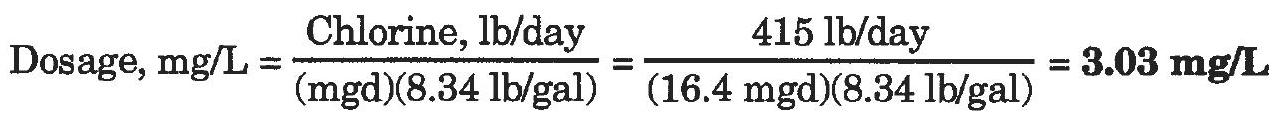
\includegraphics[max width=\textwidth]{2022_11_10_d6923b5a412978ed01fcg-36}

  \item Answer: c. 59 gal sodium hypochlorite

First, find the initial amount of water to be disinfected, $10 \%$ capacity

$$
=(1.65 \mathrm{mil} \mathrm{gal})(10 \% \div 100 \%)=0.165 \mathrm{mil} \mathrm{gal}
$$

Next, determine the number of pounds of chlorine needed by using the "pounds" equation.

Sodium hypochlorite, $\mathrm{lb}=\frac{(\mathrm{mil} \text { gal })(\text { Dosage, } \mathrm{mg} / \mathrm{L})(8.34 \mathrm{lb} / \mathrm{gal})}{\text { (\% Available chlorine) }(100 \%)}$

Sodium hypochlorite, $1 \mathrm{~b}=\frac{(0.165 \mathrm{mil} \mathrm{gal})(50.0 \mathrm{mg} / \mathrm{L})(8.34 \mathrm{lb} / \mathrm{gal})(100 \%)}{(11.8 \%)}$

Lastly, convert the pounds of sodium hypochlorite to gallons by dividing by 9.84 lb/gal.

Sodium hypochlorite, gal $=583.1 \mathrm{lb} \div 9.84 \mathrm{lb} / \mathrm{gal}=59.26$, round to $59 \mathrm{gal}$

  \item Answer: c. $11.9 \mathrm{lb}$ calcium hypochlorite

First, convert 24 in. to feet: 24 in. $\div 12$ in. per foot $=2 \mathrm{ft}$

Next, find the volume of the pipe in gallons using the following formula:

Equation: Pipe volume, gal $=(0.785)(\text { Diameter, } \mathrm{ft})^{2}($ Length, $\mathrm{ft})\left(7.48 \mathrm{gal} / \mathrm{ft}^{3}\right)$

Pipe volume, gal $=(0.785)(2.0 \mathrm{ft})(2.0 \mathrm{ft})(781 \mathrm{ft})\left(7.48 \mathrm{gal} / \mathrm{ft}^{3}\right)=18,344 \mathrm{gal}$

Next, find the number of million gallons (mil gal).

mil gal $=(18,344 \mathrm{gal})(1 \mathrm{M} \div 1,000,000)=0.018344 \mathrm{mil} \mathrm{gal}$

Then use the "pounds" equation:

Calcium hypochlorite, $\mathrm{lb}=\frac{(\mathrm{mil} \text { gal })(\text { Dosage, } \mathrm{mg} / \mathrm{L})(8.34 \mathrm{lb} / \mathrm{gal})}{(\% \text { Available chlorine })(100 \%)}$

Calcium hypochlorite, $\mathrm{lb}=\frac{(0.018344 \mathrm{mil} \mathrm{gal})(50.0 \mathrm{mg} / \mathrm{L})(8.34 \mathrm{lb} / \mathrm{gal})}{(64.3 \%)(100 \%)}=\mathbf{1 1 . 9} \mathbf{1 b}$ 24. Answer: d. $26.0 \mathrm{lb} /$ day of chlorine

First, convert the pumping rate to million gallons per day (mgd).

Equation: $\mathrm{mgd}=\frac{(\text { Pumping rate, } g p m)(1,440 \mathrm{~min} / \text { day })}{1,000,000}$

Substitute known values and solve: $\mathrm{mgd}=\frac{(428 \mathrm{gpm})(1,440 \mathrm{~min} / \mathrm{day})}{1,000,000}=0.61632 \mathrm{mgd}$

Next, find the total chlorine dose required.

Total chlorine dose, $\mathrm{mg} / \mathrm{L}=1.20 \mathrm{mg} / \mathrm{L}$ required $+3.85 \mathrm{mg} / \mathrm{L}$ demand $=5.05 \mathrm{mg} / \mathrm{L}$

Next, use the "pounds" equation to solve the problem.

Chlorine, lb/day $=(\mathrm{mgd})($ Dosage, $\mathrm{mg} / \mathrm{L})(8.34 \mathrm{lb} / \mathrm{gal})$

$=(0.61632 \mathrm{mgd})(5.05 \mathrm{mg} / \mathrm{L})(8.34 \mathrm{lb} / \mathrm{gal})$

$=25.958 \mathrm{lb} /$ day, round to $26.0 \mathrm{lb} / \mathrm{day}$

  \item Answer: b. $74.4 \mathrm{cfs}$

Equation: Number of $\mathrm{cfs}=\frac{(\mathrm{mgd})(1,000,000 \mathrm{gal})\left(1 \mathrm{ft}^{3}\right)(1 \mathrm{day})(1 \mathrm{~min})}{(1 \mathrm{mil} \mathrm{gal})(7.48 \mathrm{gal})(1,440 \mathrm{~min})(60 \mathrm{sec})}$

or: Number of $\mathrm{cfs}=\frac{(\mathrm{mgd})(1,000,000 \mathrm{gal})\left(1 \mathrm{ft}^{3}\right)(1 \mathrm{day})}{(1 \mathrm{mil} \mathrm{gal})(7.48 \mathrm{gal})(86,400 \mathrm{sec})}$

Substitute known values and solve.

Number of $\mathrm{cfs}=\frac{(48.1 \mathrm{mgd})(1,000,000 \mathrm{gal})\left(1 \mathrm{ft}^{3}\right)(1 \mathrm{day})}{(1 \mathrm{mil} \mathrm{gal})(7.48 \mathrm{gal})(86,400 \mathrm{sec})}=\mathbf{7 4 . 4} \mathrm{cfs}$

  \item Answer: c. $11.6 \mathrm{~L} / \mathrm{s}$

Equation: Flow, L/s $=\frac{(F l o w, g p m)(3.785 \mathrm{~L} / \mathrm{gal})}{60 \mathrm{sec} / \mathrm{min}}$

Flow, $\mathrm{L} / \mathrm{s}=\frac{(184 \mathrm{gpm})(3.785 \text { Liters } / \mathrm{gal})}{60 \mathrm{sec} / \mathrm{min}}=11.6 \mathrm{~L} / \mathrm{s}$

  \item Answer: c. $1.02 \mathrm{ntu}$

\begin{tabular}{|c|c|c|c|c|c|c|}
\hline
1 & 2 & 3 & 4 & 5 & 6 & 7 \\
\hline
$1.08 \mathrm{ntu}$ & $0.98 \mathrm{ntu}$ & $0.94 \mathrm{ntu}$ & $0.88 \mathrm{ntu}$ & $0.96 \mathrm{ntu}$ & $1.03 \mathrm{ntu}$ & $1.25 \mathrm{ntu}$ \\
\hline
\end{tabular}

First add all seven measurements:

$1.08+0.98+0.94+0.88+0.96+1.03+1.25=7.12 \mathrm{ntu}$

Equation: Average $=\frac{\text { Sum of measurements }}{\text { Number of measurements }}$

Average sedimentation basin $\mathrm{ntu}=\frac{7.12 \mathrm{mg} / \mathrm{L}}{7}=1.017 \mathrm{ntu}$, round to $1.02 \mathrm{ntu}$

  \item Answer: a. 410

Equation: $100 \%$ Number $=\frac{\text { (Number given })(100 \%)}{\text { Percent of given number }}$

$100 \%$ Number $=\frac{(288)(100 \%)}{70.3 \%}=409.67$, round to 410 29. Answer: d. $99 \%$ Fe removal efficiency

Equation: Percent Fe removal efficiency $=\frac{(\text { In }-\text { Out })(100 \%)}{\text { In }}$

Percent Fe removal efficiency $=\frac{(0.81-0.01)(100 \%)}{0.81}=99 \%$ Fe removal efficiency

  \item Answer: a. $3.27 \%$ soda ash slurry

Equation: Percent soda ash slurry $=\frac{\text { (Soda ash, } \mathrm{lb})(100 \%)}{\text { Soda ash, } \mathrm{lb}+(8.34 \mathrm{lb} / \mathrm{gal})(\text { Water, gal) }}$

Substitute known values and solve.

$$
\begin{aligned}
\text { Percent soda ash slurry } &=\frac{(28.2 \mathrm{lb})(100 \%)}{28.2 \mathrm{lb}+(8.34 \mathrm{lb} / \mathrm{gal})(100.0 \mathrm{gal})} \\
&=\frac{(28.2 \mathrm{lb})(100 \%)}{28.2 \mathrm{lb}+834 \mathrm{lb}}=\frac{(28.2 \mathrm{lb})(100 \%)}{862.2 \mathrm{lb}} \\
&=\mathbf{3 . 2 7 \%} \text { soda ash slurry }
\end{aligned}
$$

  \item Answer: d. $11,100 \mathrm{ft}^{2}$

First, find the square footage of the wall area.

Equation: Wall area, $\mathrm{ft}^{2}=($ Diameter, $\mathrm{ft})(\pi)($ Height, $\mathrm{ft})$; where $\pi$ equals $3.14$

Wall area, $\mathrm{ft}^{2}=(80.1 \mathrm{ft})(3.14)(24.0 \mathrm{ft})=6,036 \mathrm{ft}^{2}$

Next, find the area of the top. Note: There is no bottom exterior area.

Top area, $\mathrm{ft}^{2}=(0.785)(\text { Diameter, } \mathrm{ft})^{2}=(0.785)(80.1 \mathrm{ft})(80.1 \mathrm{ft})=5,037 \mathrm{ft}^{2}$

Total exterior surface area of tank, $\mathrm{ft}^{2}=6,036 \mathrm{ft}^{2}+5,037 \mathrm{ft}^{2}$

$=11,073 \mathrm{ft}^{2}$, round to $11,100 \mathrm{ft}^{2}$

  \item Answer: c. $99,800 \mathrm{gal}$

First, convert miles to feet:

Number of miles $=(1.43 \mathrm{miles})(5,280 \mathrm{ft} / \mathrm{mile})=7,550.4 \mathrm{ft}$

Next, convert $18.0$ inches to feet:

Number of $\mathrm{ft}=18.0$ inches $/ 12$ inches per foot $=1.50 \mathrm{ft}$

Substitute known values and solve.

Equation: Volume, gal $=(0.785)(\text { Diameter, } \mathrm{ft})^{2}($ Length, $\mathrm{ft})\left(7.48 \mathrm{gal}^{\mathrm{ft}} \mathrm{ft}^{3}\right)$

Volume, gal $=(0.785)(1.50 \mathrm{ft})(1.50 \mathrm{ft})(7,550.4 \mathrm{ft})\left(7.48 \mathrm{gal} / \mathrm{ft}^{3}\right)$

$=99,752$ gal, round to $99,800 \mathrm{gal}$

  \item Answer: b. $17.8 \mathrm{hr}$

First, find the diameter: Diameter, $\mathrm{ft}=2$ (radius) $=2(60.0 \mathrm{ft})=120 \mathrm{ft}$

Then, determine the volume of water in the storage tank.

Equation: Volume, gal $=(0.785)(\text { Diameter, } \mathrm{ft})^{2}($ Depth, $\mathrm{ft})\left(7.48 \mathrm{gal} / \mathrm{ft}^{3}\right)$

Average Tank Volume, gal $=(0.785)(120 \mathrm{ft})(120 \mathrm{ft})(25.5 \mathrm{ft})\left(7.48 \mathrm{gal}^{2} / \mathrm{ft}^{3}\right)$

$$
=2,156,125 \mathrm{gal}
$$

Next, convert mgd to gallons per day.

Flow through tank, gal/day $=(2.91 \mathrm{mgd})(1,000,000 \mathrm{gal})=2,910,000 \mathrm{gal} /$ day

Next, solve for the detention.

Equation: Detention time, $\mathrm{hr}=[($ Tank Volume $)(24 \mathrm{hr} /$ day $)] \div(\mathrm{Flow}$, gal/day) Substitute known values and solve:

Detention time, $\mathrm{hr}=[(2,156,125 \mathrm{gal})(24 \mathrm{hr} /$ day $)] \div(2,910,000 \mathrm{gal} / \mathrm{day})=17.8 \mathrm{hr}$

  \item Answer: d. $58 \mathrm{psi}$

Equation: Pressure Head, $\mathrm{ft}=($ Pressure, $\mathrm{psi})(2.31 \mathrm{ft} / \mathrm{psi})$

Rearrange to solve for pressure in psi:

Pressure, psi $=($ Pressure head, $\mathrm{ft}) \div(2.31 \mathrm{ft} / \mathrm{psi})$

Pressure, $\mathrm{psi}=134 \mathrm{ft} \div 2.31 \mathrm{ft} / \mathrm{psi}=58 \mathrm{psi}$

  \item Answer: a. $820 \mathrm{gal}$

First, convert the flow in $\mathrm{ft}^{3} / \mathrm{min}$ to gallons per minute (gpm).

$\mathrm{gpm}=\left(5.5 \mathrm{ft}^{3} / \mathrm{min}\right)\left(7.48 \mathrm{gal} / \mathrm{ft}^{3}\right)=41.14 \mathrm{gpm}$

Then determine the number of gallons that flowed through the fire hydrant.

Gallons $=(41.14 \mathrm{gpm})(20 \mathrm{~min})=822.8 \mathrm{gal}$, round to $820 \mathrm{gal}$

  \item Answer: b. $1.19 \mathrm{~g} / \mathrm{cm}^{3}$

First, convert the number of pounds to grams.

Know from conversion tables that 1 pound $=454$ grams and 1 liter $=1000.027 \mathrm{~cm}^{3}$

Number of grams $=(\mathrm{Number}$ of $\mathrm{lb})(454 \mathrm{~g} / \mathrm{lb})$

Number of grams $=(8.25 \mathrm{lb})(454 \mathrm{~g} / \mathrm{lb})=3,745.5 \mathrm{~g}$

Number of $\mathrm{cm}^{3}=\left(1000.027 \mathrm{~cm}^{3} / 1 \mathrm{~L}\right)(3.150 \mathrm{~L})=3,150.085 \mathrm{~cm}^{3}$

Equation: Density = Mass/Volume

Density $=3,745.5 \mathrm{~g} / 3,150.085 \mathrm{~cm}^{3}=1.19 \mathrm{~g} / \mathrm{cm}^{3}$

  \item Answer: b. $98.6 \%$ meter efficiency

First, convert cubic feet to gallons.

Number of gal $=\left(245.7 \mathrm{ft}^{3}\right)\left(7.48 \mathrm{gal} / \mathrm{ft}^{3}\right)=1,837.836 \mathrm{gal}$

Equation: Meter accuracy, $\%=\frac{(\text { Meter reading, gal })(100 \%)}{\text { Actual volume, gal }}$

Meter accuracy, $\%=\frac{(1,837.836 \mathrm{gal})(100 \%)}{1,863 \mathrm{gal}}=98.6 \%$ meter efficiency

  \item Answer: c. $3.3 \mathrm{mg} / \mathrm{L}$

Equation: $\mathrm{lb} / \mathrm{day}=(\mathrm{mgd})($ Dosage, $\mathrm{mg} / \mathrm{L})(8.34 \mathrm{lb} /$ day $)$

Rearrange the equation and solve for dosage.

Dosage, $\mathrm{mg} / \mathrm{L}=\frac{\mathrm{lb} / \text { day }}{(\mathrm{mgd})(8.34 \mathrm{lb} / \mathrm{gal})}=\frac{320 \mathrm{lb} / \mathrm{day}}{(11.6 \mathrm{mgd})(8.34 \mathrm{lb} / \mathrm{gal})}$

$=3.308 \mathrm{mg} / \mathrm{L}$, round to $3.3 \mathrm{mg} / \mathbf{L}$

  \item Answer: a. 678 gal of sodium hypochlorite

First, determine the number of pounds of chlorine needed by using the "pounds" equation.

Equation: Sodium hypochlorite, $\mathrm{lb}=(\mathrm{mil} \mathrm{gal})($ Dosage, $\mathrm{mg} / \mathrm{L})(8.34 \mathrm{lb} / \mathrm{gal})$ Chlorine, $\mathrm{lb}=(1.75 \mathrm{mil} \mathrm{gal})(50.0 \mathrm{mg} / \mathrm{L})(8.34 \mathrm{lb} / \mathrm{gal})=729.75 \mathrm{lb}$

Next, find the number of gallons of sodium hypochlorite.

Equation: Sodium hypochlorite, gal $=\frac{(\text { Chlorine, } \mathrm{lb})(100 \%)}{(\mathrm{lb} / \text { gal })(\% \text { Solution })}$

Substitute known values and solve.

Sodium hypochlorite, gal $=\frac{\left(729.75 \mathrm{lb} \text { of } \mathrm{Cl}_{2}\right)(100 \%)}{(8.97 \mathrm{lb} / \mathrm{gal})(12.0 \%)}=677.95 \mathrm{gal}$, round to $678 \mathrm{gal}$

  \item Answer: d. $54 \mathrm{mg} / \mathrm{L}$ chlorine

First, convert the diameter of the pipeline from inches to feet.

Number of feet $=24.0$ in. $\div 12$ in. $/ \mathrm{ft}=2.0 \mathrm{ft}$

Next, find the number of gallons by determining the volume of the pipeline.

Equation: Volume of pipe, gal $=(0.785)$ (Diameter, $\mathrm{ft})^{2}($ Length, $\mathrm{ft})$

Volume of pipe, gal $=(0.785)(2.0 \mathrm{ft})(2.0 \mathrm{ft})(427 \mathrm{ft})\left(7.48 \mathrm{gal} / \mathrm{ft}^{3}\right)=10,029 \mathrm{gal}$

Then convert number of gallons to mil gal.

Number of mil gal $=10,029 \mathrm{gal} \div 1,000,000=0.010029 \mathrm{mil} \mathrm{gal}$

Finally, calculate the dosage by rearranging the "pounds" equation.

Calcium hypochlorite, lb/day $=\frac{(\mathrm{mgd})(\text { Dosage, } \mathrm{mg} / \mathrm{L})(8.34 \mathrm{lb} / \mathrm{gal})(100 \%)}{\text { Percent available chlorine }}$

Rearrange the equation and drop the day on each side of the equation as it is not needed.

Dosage, $\mathrm{mg} / \mathrm{L}=\frac{(\text { Calcium hypochlorite, } \mathrm{lb})(65.0 \% \text { Available chlorine })}{\text { (mil gal })(8.34 \mathrm{lb} / \mathrm{gal})(100 \% \text { calcium hypochlorite })}$

$$
\begin{aligned}
&=\frac{(7.0)(65.0 \%)}{(0.010029)(8.34)(100 \%)} \\
&=54.4 \mathrm{mg} / \mathrm{L}, \text { round to } 54 \mathrm{mg} / \mathrm{L}
\end{aligned}
$$

  \item Answer: c. $7.4 \mathrm{mg} / \mathrm{L}$ sodium hypochlorite

First, convert the production rate of the well pump to mgd.

Equation: mgd $=\frac{\text { (Pumping rate) }(1,440 \mathrm{~min} / \text { day })}{1,000,000}$

$\mathrm{mgd}=\frac{(260 \mathrm{gpm})(1,440 \mathrm{~min} / \mathrm{day})}{1,000,000 \mathrm{mil} \mathrm{gal}}=0.3744 \mathrm{mgd}$

Second, convert liters/day to gallons/day.

Number of gal $=\frac{95 \text { Liters } / \text { day }}{3.785 \text { Liters } / \text { gal }}=25.1 \mathrm{gal} /$ day

Next, calculate the chlorine usage in pounds per day. Equation:

Chlorine usage, lb/day

$$
\begin{aligned}
&=\frac{(\text { Hypochlorinator flow, gal/day })\left(\% \mathrm{Cl}_{2} \text { in hypochlorite solution }\right)(8.95 \mathrm{lb} / \mathrm{gal})}{100 \%} \\
&=\frac{(25.1 \mathrm{gal} / \mathrm{day})(10.3 \%)(8.95 \mathrm{lb} / \mathrm{gal})}{100 \%}=23.14 \mathrm{lb} / \mathrm{day}
\end{aligned}
$$

Lastly, calculate the chlorine dosage using the "pounds" equation. Sodium hypochlorite, lb/day $=[(\mathrm{mgd})($ Dosage, $\mathrm{mg} / \mathrm{L})(8.34 \mathrm{lb} / \mathrm{gal})]$

Rearrange the equation to solve for dosage.

Equation: Dosage, $\mathrm{mg} / \mathrm{L}=\frac{\text { Sodium hypochlorite, } \mathrm{lb} / \text { day }}{(\mathrm{mgd})(8.34 \mathrm{lb} / \mathrm{gal})}$

Dosage, $\mathrm{mg} / \mathrm{L}=\frac{23.14}{(0.3744)(8.34)}=7.4 \mathrm{mg} / \mathrm{L}$ sodium hypochlorite


  \item Answer: a. $10.5 \mathrm{lb} /$ day of chlorine

First, convert the pumping rate to mgd.

Equation: $m g d=\frac{\text { (pumping rate, gpm })(1,440 \mathrm{~min} / \text { day })}{1,000,000}$

Substitute known values and solve:

$\mathrm{mgd}=\frac{(208 \mathrm{gpm})(1,440 \mathrm{~min} / \text { day })}{1,000,000}=0.29952 \mathrm{mgd}$

Next determine the total chlorine dosage required.

Total chlorine, $\mathrm{mg} / \mathrm{L}=$ Chlorine demand, $\mathrm{mg} / \mathrm{L}+$ chlorine residual, $\mathrm{mg} / \mathrm{L}$

Total chlorine, $\mathrm{mg} / \mathrm{L}=2.45 \mathrm{mg} / \mathrm{L}+1.75 \mathrm{mg} / \mathrm{L}=4.20 \mathrm{mg} / \mathrm{L}$

Next, use the "pounds" equation to solve the problem.

Equation: Chlorine, lb/day $=(\mathrm{mgd})($ Dosage, $\mathrm{mg} / \mathrm{L})(8.34 \mathrm{lb} / \mathrm{gal})$

Chlorine, lb/day $=(0.29952 \mathrm{mgd})(4.20 \mathrm{mg} / \mathrm{L})(8.34 \mathrm{lb} / \mathrm{gal})=\mathbf{1 0 . 5} \mathrm{lb} /$ day chlorine

  \item Answer: b. $910 \mathrm{gpm}$


Know: $1 \mathrm{hp}=33,000 \mathrm{ft}-\mathrm{lb} / \mathrm{min}$

Convert $15 \mathrm{hp}$ to $\mathrm{ft}-\mathrm{lb} / \mathrm{min}: 15 \times 33,000=495,000 \mathrm{ft}-\mathrm{lb} / \mathrm{min}$

Solve for the unknown value, $x$ :

$(65)(x \mathrm{lb} / \mathrm{min})=495,000 \mathrm{ft}-\mathrm{lb} / \mathrm{min}$

$x \mathrm{lb} / \mathrm{min}=495,000 \mathrm{ft}-\mathrm{lb} / \mathrm{min} \div 65=7,615 \mathrm{lb} / \mathrm{min}$

Now express this maximum pumping rate in gallons per minute

$7,615 \mathrm{lb} / \mathrm{min} \div 8.34 \mathrm{lb} / \mathrm{gal}=913.70 \mathrm{gpm}$, round to $910 \mathrm{gpm}$

  \item Answer: 128 gpcd

First, convert $2.98 \mathrm{mgd}$ to mil gal.

Number of gallons $=2.98 \mathrm{mgd} \times 1,000,000 \mathrm{mil} \mathrm{gal}=2,980,000 \mathrm{gal}$

Equation:

Gallons per capita per day $(\mathrm{gpcd})=$ Volume gal/day $\div$ Population served/day

gpcd $=2,980,000 \mathrm{gal} /$ day $\div 23,210$ capita/day $=128 \mathrm{gpcd}$
  
  
\end{enumerate}


\end{document}